\chapter{Desarrollo del trabajo}
\label{cap:desarrollo}

\section{Metodología experimental}

\subsection{Principios de diseño}

Toda la comparativa descansa sobre cuatro decisiones metodológicas que se fijaron antes de
ejecutar ningún experimento.

\textbf{Diseño pareado.} Cada técnica se evalúa sobre exactamente los mismos fragmentos de
audio que su línea base, en la misma ejecución y con la misma configuración de
decodificación. Esto permite comparar fragmento a fragmento en lugar de comparar dos
medias, que es lo único que proporciona algo de potencia estadística con corpus de tamaño
moderado.

\textbf{Doble criterio de significación.} Se calcula un intervalo de confianza al 95\%
para la diferencia de error mediante remuestreo por bootstrap, y un test de signos sobre
los fragmentos que cambian. Una diferencia se considera significativa solo si ambos
coinciden. El motivo es práctico: durante el trabajo apareció un caso en que el intervalo
excluía el cero por muy poco y el test de signos no lo respaldaba; interpretarlo como
efecto real habría sido forzar el dato.

\textbf{Remuestreo por fragmentos, no por palabras.} Los errores de reconocimiento se
agrupan dentro de un mismo fragmento y un mismo hablante. Tratar las palabras como
observaciones independientes estrecha el intervalo de confianza de forma artificial y
produce significación donde no la hay.

\textbf{Trazabilidad completa.} Cada resultado registra el commit del código, si el árbol
de trabajo estaba limpio, y el resumen criptográfico del manifiesto de corpus empleado. La
razón se explica en la sección~\ref{sec:incidentes}.

\subsection{Potencia estadística requerida}

Antes de interpretar ninguna diferencia hubo que responder cuánto material hace falta para
poder detectarla. Con 499 palabras de referencia, el error estándar del WER en torno al
3\% ronda 0,8 puntos, de modo que el intervalo de confianza alcanza aproximadamente
$\pm 1,5$ puntos: bajo esas condiciones, tres modelos que difieren en 0,4 puntos son
indistinguibles.

Para detectar diferencias del orden de 0,5 puntos, que es la escala en que se mueven las
técnicas de adaptación, hacen falta del orden de 30.000 palabras de referencia; unas tres
o cuatro horas de audio transcrito. La cifra es una cota optimista, porque supone errores
independientes cuando en realidad se agrupan.

Esta estimación condicionó todo lo demás: las mediciones que no la alcanzan se marcan como
no concluyentes y no se interpretan, ni a favor ni en contra.

\subsection{Corpus}

El obstáculo principal del trabajo fue localizar audio educativo en español con
transcripción de referencia fiable. La búsqueda y auditoría de candidatos se documenta en
el capítulo~\ref{cap:estado}; aquí importa el resultado: se emplearon cinco corpus de
características deliberadamente distintas, resumidos en la tabla~\ref{tab:corpus-usados}.

\begin{table}[h]
\centering
\small
\begin{tabular}{|l|l|l|r|}
\hline
\textbf{Corpus} & \textbf{Variedad} & \textbf{Registro} & \textbf{Clips} \\
\hline
\texttt{fleurs-es} & Latinoamérica & Voz leída, dominio general & 20 \\
\texttt{tedx-es} & México & Charla expositiva espontánea & 40 \\
\texttt{teleconciencia-es} & México & Divulgación científica en televisión & 1.200 \\
\texttt{mediaspeech-es} & Peninsular & Locución de medios & 40 \\
\texttt{voxpopuli-es} & Peninsular & Debate parlamentario & 400 \\
\hline
\end{tabular}
\caption{Corpus empleados en la comparativa. Ninguno es aula real; la justificación de
cada uno y sus limitaciones se detallan en el capítulo~\ref{cap:estado}.}
\label{tab:corpus-usados}
\end{table}

Ninguno de ellos es una clase grabada. Esta es la limitación de fondo del trabajo y
condiciona la validez externa de todas las conclusiones; se discute en la
sección~\ref{sec:limitaciones}.

\section{Línea base sin adaptación}

\subsection{Elección del modelo}

Se evaluaron seis tamaños de Whisper sobre el mismo material. La
figura~\ref{fig:modelos} muestra el compromiso entre calidad y coste, y la
tabla~\ref{tab:baseline-corpus} recoge el detalle por corpus.

\begin{figure}[h]
\centering
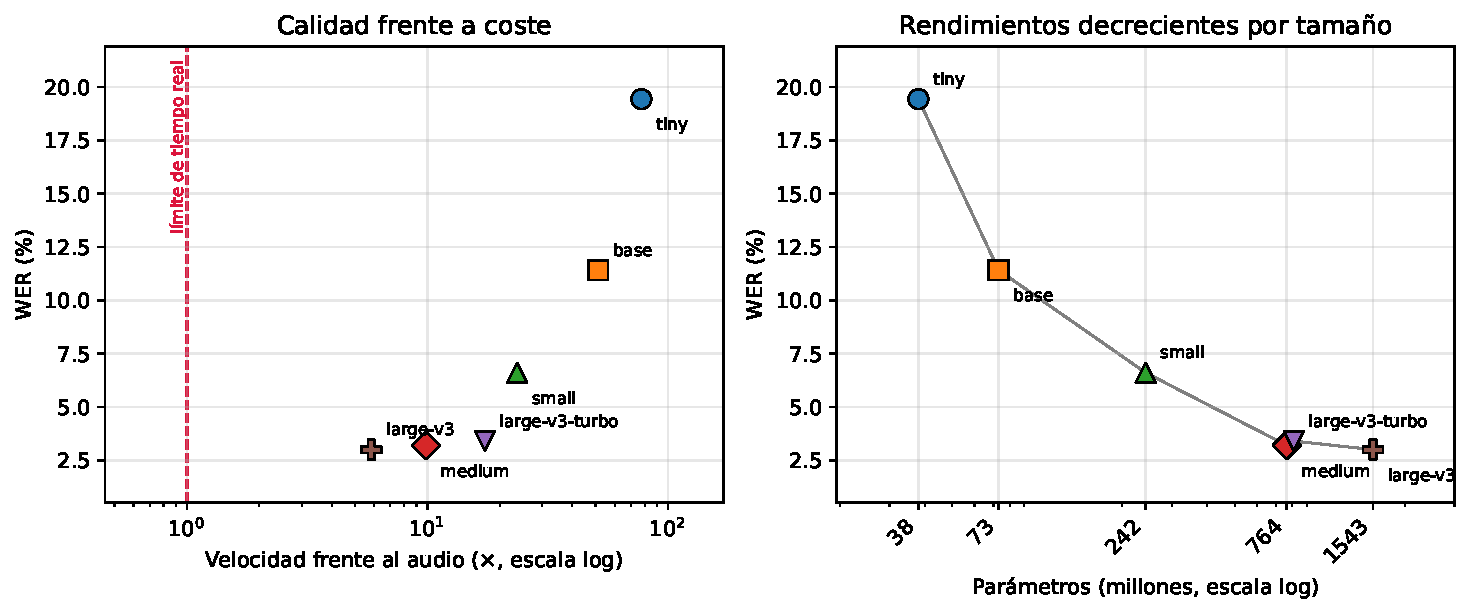
\includegraphics[width=\textwidth]{figuras/baseline_modelos_fleurs_es_fallback.pdf}
\caption{Calidad frente a coste y rendimientos decrecientes por tamaño de modelo. La línea
vertical marca el límite de tiempo real. Generada desde los datos de ejecución.}
\label{fig:modelos}
\end{figure}

% GENERADO AUTOMATICAMENTE por research/eval/report/tabla_corpus.py
% No editar a mano.
\begin{table}[h]
\centering
\small
\begin{tabular}{|l|l|l|r|r|r|r|r|r|r|}
    \hline
    \textbf{Corpus} & \textbf{Variedad} & \textbf{Registro} & \textbf{tiny} & \textbf{base} & \textbf{small} & \textbf{medium} & \textbf{large--v3--turbo} & \textbf{large--v3} & \textbf{$\Delta$ tildes} \\
    \hline
    \texttt{fleurs-es} & Latinoamérica & Leída, enciclopédica & 19.44 & 11.42 & 6.61 & 3.21 & 3.41 & 3.01 & -- \\
    \texttt{tedx-es} & México & Charla espontánea & -- & -- & 12.13 & 10.22 & 11.12 & -- & $-$3.48 \\
    \texttt{teleconciencia-es} & México & Divulgación científica & -- & -- & 23.42 & 18.61 & 22.26 & -- & $-$5.11 \\
    \texttt{mediaspeech-es} & Peninsular & Medios, locución & -- & -- & 15.94 & 14.72 & 15.60 & -- & $-$1.70 \\
    \texttt{voxpopuli-es} & Peninsular & Parlamentario & -- & -- & 12.01 & 10.44 & 11.53 & -- & $-$0.07 \\
    \hline
\end{tabular}
\caption{WER (\%) de los modelos Whisper sin adaptar segun corpus, con normalizacion
basica. La columna $\Delta$ tildes indica cuanto baja el WER de \texttt{medium} al
ignorar la acentuacion: valores altos delatan referencias con tildes omitidas (R11), no
mejor reconocimiento.}
\label{tab:baseline-corpus}
\end{table}


Dos observaciones condicionan el resto del trabajo.

La primera: en material de habla espontánea, aumentar el tamaño del modelo deja de
compensar. Entre \texttt{medium} y \texttt{large-v3-turbo} la diferencia es nula, y entre
\texttt{small} y \texttt{medium} apenas 1,5 puntos sobre el corpus más difícil, frente a
los 3,2 que separan los mismos modelos en voz leída. El margen que queda no está en el
tamaño; ese es precisamente el supuesto que motiva estudiar la adaptación.

La segunda: lo que domina el error no es la variedad dialectal sino el registro. A registro
equivalente, el español peninsular y el mexicano dan cifras casi idénticas: 10,44\% frente
a 10,22\%. Lo que lleva el error del 3\% al 23\% es leer un texto frente a hablar de forma
espontánea.

\subsection{El modelo elegido y por qué no es el más rápido}

La primera lectura recomendaba \texttt{large-v3-turbo}: igualaba a \texttt{medium} en tasa
de error y era el doble de rápido. Esa lectura ignoraba el modo de fallo.

Contabilizando las salidas anómalas, entendidas como transcripciones con menos de un cuarto
de las palabras esperadas, \texttt{turbo} produjo tres sobre 180 fragmentos y
\texttt{medium} ninguna. Y no son truncamientos inocuos: en varios fragmentos el modelo
emitió una frase fluida, gramatical y plausible en el dominio que no guardaba relación con
lo dicho.

Para un sistema de accesibilidad ese criterio pesa más que unas décimas de tasa de error.
Un subtítulo ausente se nota; uno inventado, no: el alumno con discapacidad auditiva no
tiene forma de detectarlo porque se lee perfectamente bien. Se eligió \texttt{medium}.

\section{Comparativa de técnicas de adaptación}

% GENERADO AUTOMATICAMENTE por research/eval/report/tabla_tecnicas.py
% No editar a mano.
\begin{table}[h]
\centering
\small
\begin{tabular}{|l|l|r|r|r|c|r|c|}
    \hline
    \textbf{Técnica} & \textbf{Corpus} & \textbf{WER base} &
    \textbf{WER téc.} & \textbf{$\Delta$ (pp)} & \textbf{IC 95\%} &
    \textbf{$p$} & \textbf{Signif.} \\
    \hline
    Prompting contextual & \texttt{tedx-es} & 10.15 & 9.96 & -0.19 & [-0.61, +0.00] & 1.000 & No \\
    Prompting contextual & \texttt{teleconciencia-es} & 18.79 & 19.14 & +0.35 & [-0.52, +1.42] & 0.012 & No \\
    Prompting contextual & \texttt{voxpopuli-es} & 9.99 & 9.60 & -0.39 & [-1.14, +0.45] & 0.375 & No \\
    Post-corrección con LLM & \texttt{teleconciencia-es} & 19.55 & 22.77 & +3.23 & [+2.66, +3.84] & 0.000 & Sí \\
    Post-corrección con LLM & \texttt{voxpopuli-es} & 12.50 & 12.15 & -0.35 & [-1.69, +1.12] & 1.000 & No \\
    \hline
\end{tabular}
\caption{Efecto de cada técnica de adaptación sobre el WER (\%), con diseño pareado.
$\Delta$ negativo indica mejora. El intervalo de confianza se obtiene por bootstrap
remuestreando clips; $p$ corresponde al test de signos sobre los clips que cambian.}
\label{tab:comparativa-tecnicas}
\end{table}


\subsection{Prompting contextual}

La técnica aporta al decodificador un glosario del dominio como contexto previo. El
glosario se extrae de fragmentos disjuntos de los que se evalúan; construirlo con las
transcripciones de evaluación sería una fuga de información y cualquier mejora medida
sería falsa.

El resultado no es concluyente, y lo interesante es que no lo es de dos maneras
incompatibles: sobre el corpus mexicano el efecto es de $+0{,}35$ puntos y sobre el
peninsular de $-0{,}37$. En ambos casos los dos criterios estadísticos discrepan entre sí.
Un efecto cuyo signo se invierte entre corpus y cuyas pruebas no coinciden no es un efecto
pequeño: es la firma de la ausencia de efecto.

La métrica de terminología matiza esa conclusión. Sobre el corpus grande, el prompting
aumenta la cobertura de términos del glosario en 1,42 puntos mientras reduce su precisión
en 1,04: recupera términos que antes se perdían, y a cambio empieza a introducirlos donde
no los hay. El desglose de errores lo confirma desde el otro lado, con 66 sustituciones
menos pero 43 inserciones y 74 omisiones más. El modelo acierta más veces \emph{qué}
palabra es, y falla más veces \emph{si} la palabra estaba.

\subsection{Post-corrección con un modelo de lenguaje local}

Un modelo de lenguaje corrige la transcripción ya producida. La salida del reconocedor
queda fija, de modo que la única variable es la corrección.

La técnica degrada de forma significativa, y el resultado se replicó sobre dos corpus con
características opuestas: $+3{,}23$ puntos sobre referencias con erratas y $+1{,}18$ sobre
referencias verificadas manualmente. La diferencia de magnitud entre ambos es en sí misma
informativa: buena parte del efecto medido inicialmente era un artefacto de la calidad de
la referencia, y la cifra defendible es la del corpus limpio.

El mecanismo se observa directamente en las transcripciones. El modelo sustituye palabras
por sinónimos más precisos, expande siglas, corrige la gramática del hablante y completa lo
que interpreta como intención:

\begin{quote}
\texttt{cirugía} $\rightarrow$ \texttt{quirófano} \\
\texttt{Instituto de Tecnología de la UNAM} $\rightarrow$ \texttt{Universidad Nacional
Autónoma de México (UNAM)} \\
\texttt{atiendan a como un tipo terapia} $\rightarrow$ \texttt{atiendan cómo un tipo de
terapia}
\end{quote}

Cada una de esas ediciones mejora el texto como pieza escrita y lo empeora como
transcripción; son objetivos en conflicto, y un modelo entrenado para generar lenguaje
natural optimiza el primero.

El caso más ilustrativo es otro: en un fragmento, el corrector sustituyó el nombre de una
persona por el nombre de una enfermedad, quedándose con el tema del programa. El resultado
es fluido, gramatical y completamente falso.

Conviene declarar una limitación de este resultado. La primera versión de las instrucciones
dadas al corrector era puramente prohibitiva, y con ella la técnica quedó inerte: ningún
fragmento modificado a nivel de palabra, y errores evidentes sin corregir. Añadir ejemplos
de qué sí debía corregirse la activó. El experimento mide, por tanto, una implementación
concreta y no la técnica en abstracto.

\subsection{Ajuste fino con LoRA}

Es la única de las tres que modifica los pesos del modelo, y la única que mejora de forma
concluyente: 1,23 puntos de reducción del error, con intervalo de confianza
$[-1{,}75, -0{,}77]$ y ambos criterios de acuerdo. El entrenamiento empleó 1.500 fragmentos
(4,64 horas) durante 15,8 minutos, y produjo un adaptador de 18,9~MB frente a los 3~GB del
modelo completo.

La partición de entrenamiento y la de evaluación provienen de divisiones oficiales
distintas del mismo corpus, de modo que la separación no depende de un reparto propio.

El resultado exige un matiz. La caída del error sobre contenido crítico, de 17,52\% a
6,12\%, procede casi toda de los numerales, y el motivo se ve contando dígitos: la
referencia escribe los números en letra y el modelo base los escribía en cifra. El ajuste
fino aprendió esa convención de transcripción. Es adaptación real, pero de estilo y no de
reconocimiento acústico. Un fragmento lo ilustra: donde la referencia dice
\texttt{uno seiscientos ochenta y seis}, el modelo base escribió \texttt{1 686} y el
ajustado \texttt{cero cero seis}; acertó el formato y falló el número, y ambas métricas lo
premiaron. Descontando los numerales, la mejora sobre contenido crítico es real pero
modesta: de 7,7\% a 6,2\%.

\section{El WER no basta para evaluar accesibilidad}

Cuatro observaciones independientes, obtenidas a lo largo del trabajo, apuntan a la misma
conclusión: la métrica habitual del campo oculta precisamente los fallos que perjudican al
usuario final.

\textbf{Contenido crítico.} Sobre el corpus grande, con una tasa de error de palabra del
18,61\%, que suena aceptable, el sistema pierde o altera el 28\% de las negaciones e
introduce trece que nadie pronunció. Perder una preposición se reconstruye por contexto;
perder un \emph{no} invierte la frase. El WER cuenta ambos errores igual.

\textbf{Alucinaciones fluidas.} Los modelos producen ocasionalmente texto verosímil y falso
en lugar de fallar de forma visible. Al tratarse de salidas gramaticales y coherentes con
el dominio, ni el WER agregado ni el usuario final las detectan.

\textbf{Terminología.} El prompting contextual no mueve el WER pero sí recupera términos
del glosario. Sin una métrica específica, la técnica habría parecido completamente
inocua cuando en realidad tiene un efecto dirigido.

\textbf{Duplicación por solapamiento.} Un defecto de implementación que multiplicaba texto
en las fronteras entre ventanas elevaba el WER por encima del 100\%, pero pasó inadvertido
en las pruebas automáticas y solo se detectó al leer una transcripción real.

De estas observaciones surgieron dos instrumentos complementarios: una métrica de
cobertura y precisión sobre la terminología del dominio, y otra que contabiliza los errores
sobre negaciones, numerales y cuantificadores, es decir, sobre las unidades cuya
alteración cambia el significado y no solo la forma.

\section{Desarrollo de la aplicación}

\subsection{Arquitectura}

El sistema separa estrictamente el núcleo investigador del aplicado: la aplicación depende
de una interfaz de reconocimiento y no del código de los experimentos. Esa frontera permitió
incorporar el adaptador ganador al sistema desplegado sin modificar una sola línea de la
aplicación.

La topología es de un emisor y múltiples receptores. El docente captura desde su equipo;
el alumnado únicamente visualiza. Todo el reconocimiento ocurre una vez en el servidor,
con independencia del número de clientes conectados: un diseño donde cada cliente
transcribiera exigiría una unidad de cálculo por alumno, lo que contradice el objetivo de
que un centro pueda desplegarlo.

El acceso queda restringido a la red local por la propia aplicación, que rechaza cualquier
conexión ajena a un rango privado. Se difunde audio de aula con voces identificables; la
restricción no puede depender de que nadie configure mal un reenvío de puertos.

\subsection{Troceado del audio: latencia frente a calidad}

El subtitulado en vivo no puede esperar a que termine la intervención: hay que trocear. La
pregunta es cuánto cuesta cada segundo de latencia que se ahorra.

Un barrido de tamaños de ventana mostró que trocear cada $N$ segundos degrada de forma
sustancial: con ventanas de tres segundos el error casi se duplica respecto a transcribir
el fragmento completo. El motivo son los cortes arbitrarios, que caen en mitad de palabra
o de sintagma justo donde el modelo necesita contexto.

Esa hipótesis se contrastó cortando en los silencios en lugar de por reloj. Los resultados
aparecen en la tabla~\ref{tab:vad}.

\begin{table}[h]
\centering
\small
\begin{tabular}{|l|r|r|r|}
\hline
\textbf{Estrategia} & \textbf{WER} & \textbf{Duración media} & \textbf{p95} \\
\hline
Ventana fija, tope 3~s & 19,85\% & 2,68~s & 3,00~s \\
Silencios, tope 8~s & \textbf{12,48\%} & 2,93~s & 5,92~s \\
Sin trocear (referencia) & 10,44\% & --- & --- \\
\hline
\end{tabular}
\caption{Segmentación por silencios frente a ventana fija, a latencia media equivalente.}
\label{tab:vad}
\end{table}

A latencia media prácticamente idéntica, segmentar por silencios reduce el error 7,4
puntos y se queda a dos del techo que marca transcribir sin trocear. El mecanismo se ve en
las duraciones: con tope de ocho segundos, la segmentación por pausas produce segmentos de
2,9 segundos de media porque el tope casi nunca se alcanza. El resultado son segmentos
cortos y completos, en lugar de cortos y partidos.

El precio es la previsibilidad: el percentil 95 pasa de 3,00 a 5,92 segundos. La latencia
media mejora, pero el peor caso empeora; en accesibilidad esa distinción importa y ambas
cifras deben reportarse.

Se comprobó además si arrastrar la transcripción anterior como contexto entre ventanas
mejoraba los cortes. No aporta: el efecto es de $+0{,}14$ puntos con ventana fija y
$+0{,}61$ con segmentación por silencios. La explicación encaja con lo anterior: cuando los
cortes caen en pausas, cada segmento ya es una unidad coherente, de modo que el contexto no
añade información que falte pero sí arrastra los errores del segmento previo.

\subsection{Requisito de hardware}

Ejecutar el reconocimiento en unidad de procesamiento gráfico no es una comodidad sino un
requisito: el modelo elegido alcanza 8,1 veces la velocidad del audio en GPU y solo 1,6 en
procesador convencional. Descontado el troceado, esa segunda cifra no llega a tiempo real.

\subsection{Robustez frente al ruido de aula}

Se caracterizó la degradación mediante ruido añadido de dos tipos: blanco, estacionario, y
murmullo sintetizado superponiendo voces del propio corpus. Los resultados aparecen en la
tabla~\ref{tab:ruido}.

\begin{table}[h]
\centering
\small
\begin{tabular}{|l|r|r|}
\hline
\textbf{Relación señal-ruido} & \textbf{Ruido blanco} & \textbf{Murmullo} \\
\hline
Audio limpio & 10,44\% & 10,44\% \\
20~dB & 10,50\% & 11,66\% \\
15~dB & 10,57\% & 11,19\% \\
10~dB & 13,23\% & 12,41\% \\
5~dB & 13,98\% & 14,26\% \\
0~dB & 16,85\% & \textbf{36,02\%} \\
\hline
\end{tabular}
\caption{Degradación frente al ruido según relación señal-ruido y tipo de ruido.}
\label{tab:ruido}
\end{table}

Hasta 15~dB la degradación es despreciable, lo que sitúa un micrófono de solapa corriente
en zona segura y permite formular el requisito de captación en términos concretos. Pero el
fallo no es gradual: entre 5 y 0~dB con murmullo el error se triplica, mientras que el
ruido blanco al mismo nivel apenas lo altera. La diferencia confirma el mecanismo: lo que
arruina el reconocimiento no es la energía del ruido sino que comparta espectro con la voz.
Seis voces de fondo enmascaran lo que un ventilador no, y por eso los supresores de ruido
convencionales, diseñados para ruido estacionario, no resuelven el problema del aula.

\section{Incidentes metodológicos}
\label{sec:incidentes}

Varios de los resultados anteriores estuvieron a punto de ser erróneos. Se documentan
porque comparten una característica que los hace peligrosos: en todos los casos el sistema
seguía funcionando y produciendo cifras verosímiles.

\textbf{La configuración de decodificación como factor de confusión.} Con decodificación
voraz, uno de los modelos truncaba seis de cada cuarenta fragmentos y llegaba a emitir
frases plausibles del dominio en lugar del contenido real; su tasa de error subía de 11,5\%
a 24,2\%. Comparar técnicas sin fijar esta configuración habría medido artefactos de
decodificación en lugar del efecto de la adaptación. Desde entonces, la decodificación
forma parte del nombre de cada fichero de resultados.

\textbf{Sobrescritura del corpus.} Al ampliar un corpus de 40 a 1.200 fragmentos se
sobrescribió su manifiesto; los resultados anteriores seguían apuntando a un fichero cuyo
contenido ya era otro, y nada lo delataba. La corrección fue doble: registrar el resumen
criptográfico del manifiesto en cada resultado, para detectar la discrepancia, y permitir
que varias muestras de la misma fuente convivan, para prevenirla.

\textbf{Un entrenamiento roto que no daba error.} El primer ajuste con LoRA terminó
correctamente, guardó su adaptador y produjo métricas evaluables, con la función de pérdida
estancada en 6,87 y subiendo entre épocas. La causa era que el preparador de lotes
descartaba un identificador de token equivocado, de modo que el decodificador recibía
duplicado el marcador de inicio. Corregido, la pérdida cayó a 0,21. De no haberse
detectado, la evaluación habría mostrado que el ajuste fino destroza el modelo, con
intervalo estrecho y significación respaldando un artefacto.

\textbf{Ajustar sobre referencias defectuosas.} Uno de los corpus disponibles omite las
tildes de forma sistemática. Entrenar sobre él habría enseñado al modelo a no acentuar y,
medido contra esas mismas referencias, la tasa de error \emph{habría mejorado}: se habría
optimizado hacia el error con la métrica dando la razón.

\textbf{Un preprocesado que anula la segmentación.} Al probar la aplicación con micrófono
real, casi todos los segmentos se cerraban por agotar el tope en lugar de por pausa. La
causa no estaba en el algoritmo sino en el control automático de ganancia del navegador:
al callar el hablante sube la ganancia, amplifica el ruido de fondo y la energía nunca
desciende lo suficiente. Es un efecto que ningún experimento sobre audio grabado podía
detectar, porque solo existe cuando hay un micrófono y un navegador de por medio.

Este último incidente ilustra la relación entre los dos núcleos del trabajo mejor que
cualquier argumento: la investigación proporcionó a la aplicación su criterio de diseño,
y la aplicación descubrió una condición sin la cual ese criterio no se cumple.
